\documentclass[8pt, twocolumn]{article}


\usepackage{url}
\usepackage[hyperfootnotes=false]{hyperref}
\usepackage[font=footnotesize,labelfont=bf]{caption}
\usepackage{graphicx}
\usepackage{subcaption}
\usepackage{setspace}
\usepackage[top=0.6 in, bottom=0.7 in, left=0.7in, right=0.7in]{geometry}
\usepackage{setspace}
\usepackage{vector}
\usepackage{amsmath}
\usepackage{amssymb}
\usepackage{tgtermes}
\DeclareGraphicsExtensions{.pdf,.png,.jpg}

\usepackage{epstopdf}

\begin{document}
\title{Deuteron Electro-Disintegration at Very High Missing Momenta}
\author{Carlos Yero \\Major Advisor: Dr. Werner Boeglin}
\date{October 2016}
\maketitle

\section{Motivation} 
The deuteron ($^{2}$H) was discovered in 1931 by Harold Urey, and
it remained a mystery until the discovery of the neutron by 
James Chadwick the following year \cite{boeglin1}. Since then, the deuteron 
has been under intensive research in an attempt to understand 
what binds the atomic nucleus. Being a simple $np$ bound 
state, the deuteron serves as a starting point to study the
strong nuclear force at the subfermi level which is currently
not well understood. At such small internucleon distances 
the NN (nucleon-nucleon) potential is expected to exhibit a repulsive core in which 
the interacting nucleon pair begins to overlap. The overlap is 
directly related to two-nucleon short range correlations (SRC) observed in $A\geq2$
nuclei \cite{boeglin3}. Short-distance studies of the deuteron are
also important in determining whether or to what extent the
description of nuclei in terms of nucleon/meson degrees of 
freedom must be supplemented by the inclusion of explicit
quark effects \cite{boeglin4}. \\   
\indent In nuclear structure studies in general, electron-nucleon scattering serves as the most valuable 
tool since the interaction is described by Quantum Electro-Dynamics (QED), which is 
well-understood and capable of making accurate predictions. Electron scattering experiments can 
be separated into inclusive or exclusive scattering experiments. In the first of these, only the electron is 
detected in the final state (single-arm experiments), and so one studies the nucleus in question by
integrating over all possible final states \cite{boeglin2}. In the exclusive type, one or more 
particles are detected in coincidence with the scattered electron which allows one to investigate 
properties unique to the specific reaction in question. In deuteron electro-disintegration, for example,
one detects the scattered electron in coincidence with a proton and the missing neutron is 
reconstructed from four-momentum conservation. This reaction proves to be the most direct way of probing the 
internal structure of the deuteron since it is possible to deduce the internal momentum of the nucleons
from the neutron missing momentum. \\ 
\indent With the 12 GeV Upgrade at Jefferson Lab, the short-range ($\leq$ 1 fm) structure of the deuteron will become experimentally 
accessible via data on the deuteron wavefunction beyond relative internal momenta of 400 MeV/c.
At such high energies, one will be able to probe if effects due to 
Quantum Chromodynamics (QCD) start playing a more significant role \cite{boeglin3}. 
\section{Theoretical\hspace{1.5mm}Framework\hspace{1.5mm}of D(e,e'p)n}
Deuteron electro-disintegration can be pictorially described by a Feynmann diagram 
(See Figure \ref{fig:Figure1})
\begin{figure}[h]
  \centering
  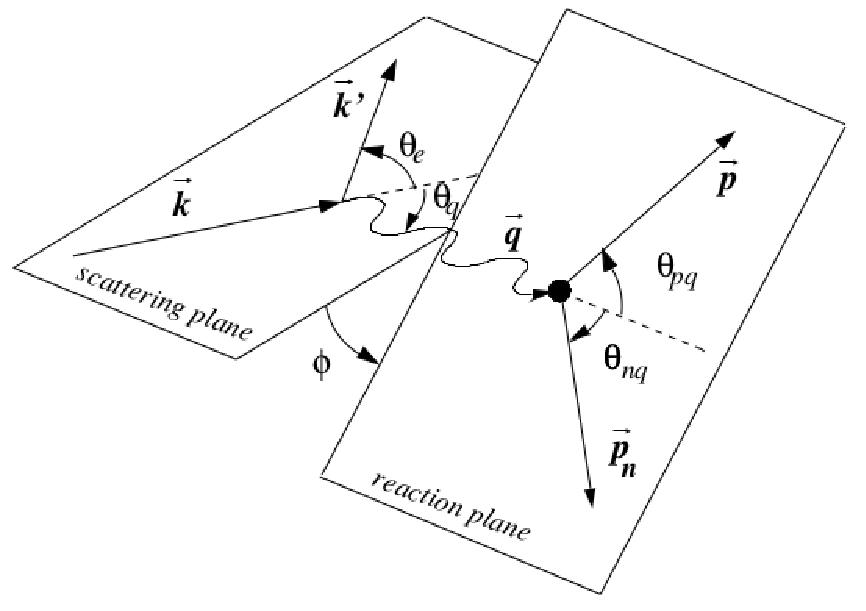
\includegraphics[width=2.8in, height=1.8in]{feynmann.pdf}
  \caption{Feynmann diagram of deuteron electro-disintegration}
  \label{fig:Figure1}
\end{figure}
\noindent where the incoming electron interacts with the stationary deuteron to first order approximation via the exchange of a virtual
photon. Given the relatively weak coupling constant for this process, higher order Feynmann diagrams involving multiple photon exchanges 
may be neglected. The interaction of the virtual photon with the deuteron is best described by the general unpolarized (e,e'p) cross section,\cite{boeglin2}
\begin{equation} \label{eq:1}
\begin{aligned}
&\frac{d^{6}\sigma}{d\omega d\Omega_{e}dT_{p}d\Omega_{p}} = \sigma_{Mott}(v_{L}R_{L}+v_{T}R_{T}+ \\
&v_{LT}R_{LT}\cos\phi+v_{TT}R_{TT}\cos 2\phi)
\end{aligned}
\end{equation}
where $\sigma_{Mott}$ is the Mott cross section describing electron scattering off an infinitely massive,
spinless point charge. The quantities ($v_{i}, v_{ij}$) are dependent on electron kinematics (i.e., q, $Q^{2}$, $\theta_{e}$) 
and the functions ($R_{i}, R_{ij}$) are nuclear response functions and depend on nuclear charge and
current density operators \cite{hari}. \\
\indent In the simplest approximation, the virtual photon couples to the proton which is ejected
from the nucleus without further interaction with the recoiling nucleus which carries a momentum $\mathbf{p_{m}}=-\mathbf{p_{i,p}}$. Both final state proton and
neutron are assumed to be plane waves (free particles), hence the name Plane Wave Impulse Approximation (PWIA). (See Figure \ref{fig:Figure2}) 
\begin{figure}[h]
  \centering
  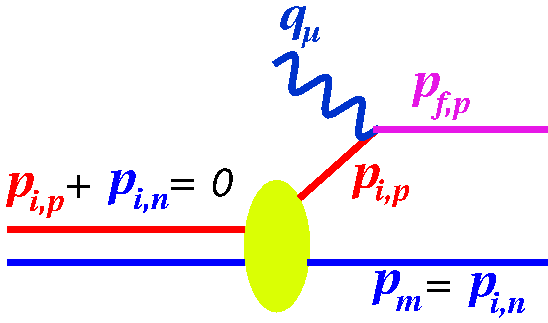
\includegraphics[width=1.5in, height=1in]{PWIA.pdf}
  \caption{Feynmann diagram for PWIA, where the proton(red) is knocked by the photon, and the
neutron(blue) scatters as a spectator}
  \label{fig:Figure2}
\end{figure} \\  
\noindent From the PWIA assumptions, the general (e,e'p) cross section (See Eq.\ref{eq:1}) can be factorized into
\begin{equation} \label{eq:2}
\begin{aligned}
\sigma_{exp}\equiv\frac{d^{6}\sigma}{d\omega d\Omega_{e}dT_{p}d\Omega_{p}} = K \sigma_{ep} S(E_{m}, p_{m}) 
\end{aligned}
\end{equation}
where $K$ is a kinematic factor, $\sigma_{ep}$ describes the elementary electron-proton cross section
for electron scattering off a bound proton, and $S(E_{m},p_{m})$ is a spectral function which
can be interpreted as the probability of finding a recoiling nucleon with missing energy and 
momentum \cite{hari}. \\
%\indent In addition to the PWIA, the virtual photon may also couple to the neutron. This process, known as the
%Plane Wave Born Approximation (PWBA), is enough to break factorization of the (e,e'p) cross section 
%provided the neutron carries a significant portion of the transferred energy and momentum comparable to that of the proton.\\
\indent In reality, the final state particles undergo subsequent interactions resulting in re-scattering of the proton and neutron.
This process is known as Final State Interactions (FSI) (See Figure \ref{fig:Figure3}) and has been shown to have a significant contribution
to the experimental cross section at high missing momenta (See Figure \ref{fig:Figure7}), therefore one cannot be confident that at
large missing momenta, the high momentum component of the deuteron will be probed \cite{ibrahim}.
\begin{figure}[h]
  \centering
  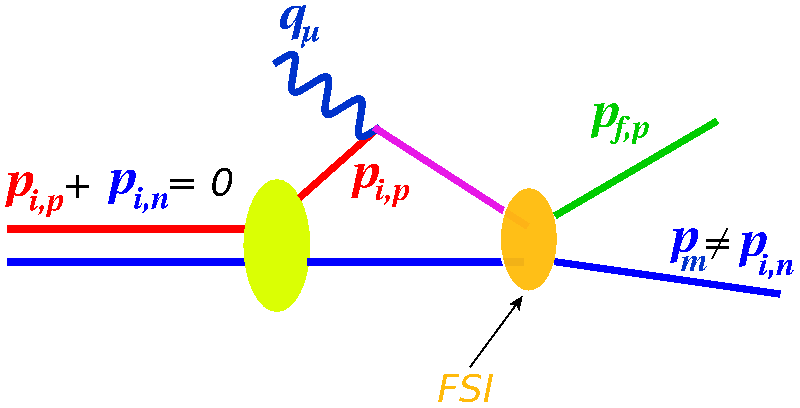
\includegraphics[width=1.8in, height=1in]{FSI.pdf}
  \caption{Feynmann diagram for FSI, where the proton(red), after excitation by the photon, 
undergoes subsequent interactions (orange) with the neutron(blue) resulting in a re-scattering
of both final state particles.}
  \label{fig:Figure3}
\end{figure} \\
\indent Another possibility is that the photon may couple to the virtual 
meson being exchanged between the nucleons (Meson Exchange Currents or MEC). (See Figure \ref{fig:Figure4})
\begin{figure}[h]
  \centering
  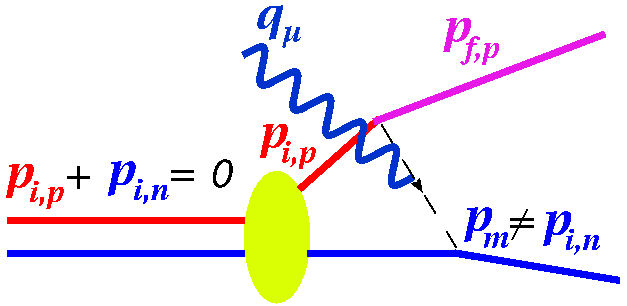
\includegraphics[width=1.6in, height=0.8in]{MEC.pdf}
  \caption{Feynmann diagram for MEC, where the virtual photon couples to the
exchange meson (dashed line) causing the spectator neutron(blue) to re-scatter off 
the proton(red)}
  \label{fig:Figure4}
\end{figure}\\
\noindent Or, the photon may excite either nucleon in the deuteron (Isobaric Configuration or IC). (See Figure \ref{fig:Figure5}) 
\begin{figure}[h]
  \centering
  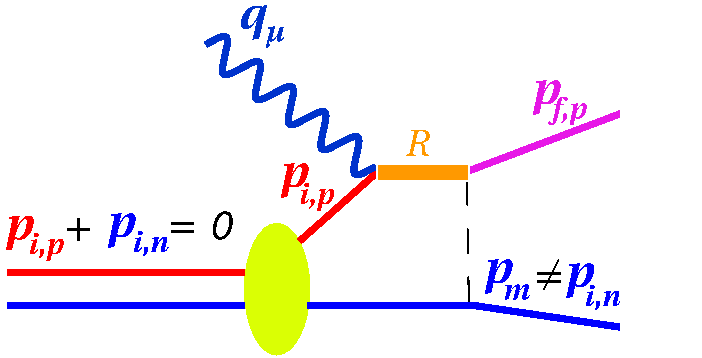
\includegraphics[width=1.8in, height=1in]{IC.pdf}
  \caption{Feynmann diagram for IC, where the proton(red) is excited by the photon
into an intermediate state (orange) R. The excited state decays and rescatters off the
neutron(blue) in the process}
  \label{fig:Figure5}
\end{figure} \\
\indent It is possible to extract the reduced cross section $\sigma_{red}$ by dividing Eq. \ref{eq:2} 
by $K$ and $\sigma_{ep}$ and integrating over the missing energy to obtain
\begin{equation} \label{eq:3}
\sigma_{red} \equiv S(p_{m}) = \frac{\sigma_{exp}}{K\sigma_{ep}}
\end{equation}
If the PWIA were valid, the reduced cross section would be the momentum distribution
inside the deuteron, therefore it is important to study at which kinematic
settings competing processes are suppressed (MEC, IC), or at least 
under control (FSI) \cite{boeglin3}.\\
\indent FSI are well described by the Generalized Eikonal Approximation (GEA) in the high energy limit($Q^{2}\geq1$ (GeV/c)$^{2}$).
The GEA predicts a strong angular dependence of FSI as a function of the scattering angle $\theta_{nq}$
between spectator nucleon and virtual photon, which opens a kinematic window
at which FSI are reduced \cite{boeglin1}. (See Figure \ref{fig:Figure6})
 \begin{figure}[h]
  \centering
  \includegraphics[width=2.9in, height=1.9in]{FSI_ang_dist.eps}
  \caption{Ratio of FSI/PWIA cross-section vs. scattering angle between 
  spectator neutron and virtual photon, $\theta_{nq}$, for various missing momenta up to
  1 GeV/c \cite{boeglin1}.}
  \label{fig:Figure6}
\end{figure}\\
\indent A previous Hall A experiment (E01-020) \cite{ulmer} at $Q^{2}=3.5$ (GeV/c)$^{2}$ 
and various $\theta_{nq}$ examined the effect of FSI for missing momenta 
up to 0.55 GeV/c. The experiment verified the strong anisotropy of FSI 
as predicted by GEA. Furthermore, there was shown to be a good  
agreement between data and theory for reduced cross sections at 
large missing momenta ($\geq$ 300 MeV/c) for smaller $\theta_{nq}$ angles without the 
inclusion of FSI. (See Figure \ref{fig:Figure7} (a) and (b))   
\begin{figure}[h]
  \centering
  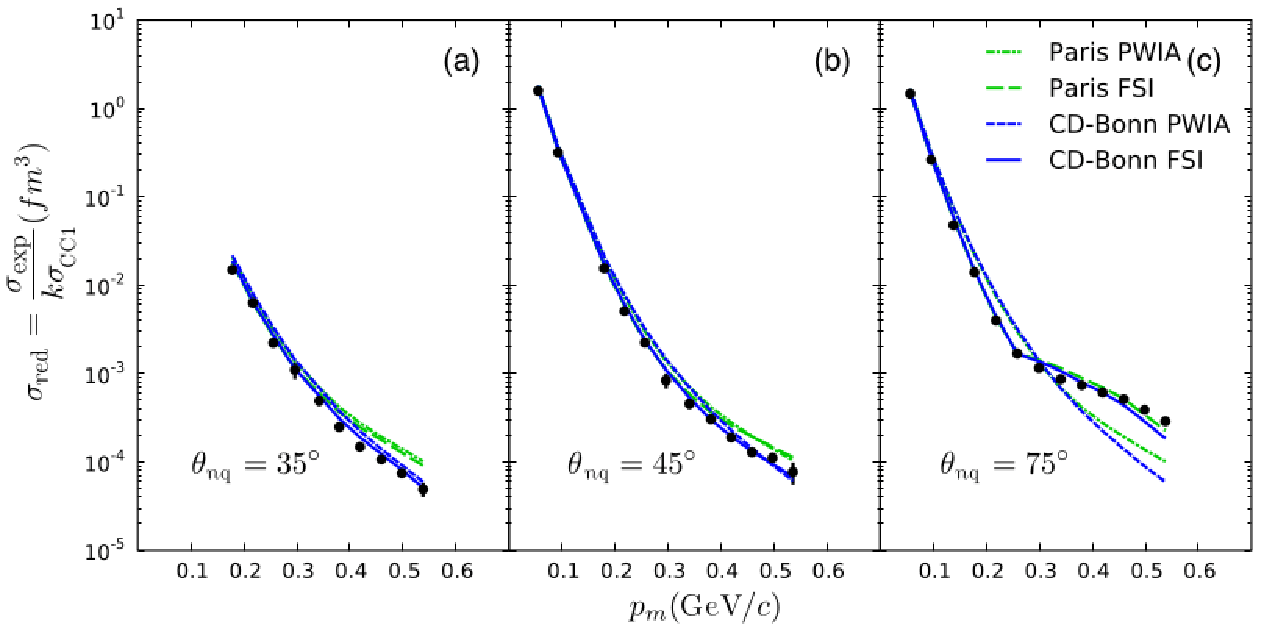
\includegraphics[width=3.7in, height=2.0in]{red_cross.pdf}
  \caption{Reduced cross-section $\sigma_{red}$ vs. missing momenta $p_{m}$ for angles (a) $\theta_{nq}=35^{\circ}$, (b) $\theta_{nq}=45^{\circ}$ and (c) $\theta_{nq}=75^{\circ}$ \cite{ulmer}.}
  \label{fig:Figure7}
\end{figure}
\vspace{-0.6cm}
\section{Project Status}
The Deuteron Electro-Disintegration at Very High Missing Momenta  
experiment (E12-10-003) will be the third of four commissioning experiments and
is scheduled to run on April 2017 on Hall C, Jefferson Lab. The experiment will extend the
the missing momentum range studied in E01-020 from  $p_{m}=0.5$ GeV/c to $p_{m}=1.0$ GeV/c
at a $Q^{2}=4.25$ (GeV/c)$^{2}$ and $x_{Bj}$=1.35 for $\theta_{nq}=40^{\circ}$
where FSI are expected to be reduced. (See Figure \ref{fig:Figure6}) The main focus of E12-10-003
will be to extract the unpolarized D(e,e'p)n cross section and momentum distribution for unexplored
large missing momentum regions at high $Q^{2}$. Various physics simulations have been performed
that predict the D(e,e'p)n experimental cross section as a function of missing momenta from 0.44 to 1.0 GeV/c for the abovementioned kinematic settings. 
The expected results and beam times for each momentum
setting are shown in Figure \ref{fig:Figure8}\cite{mark_pres}.
\begin{figure}[h]
  \centering
  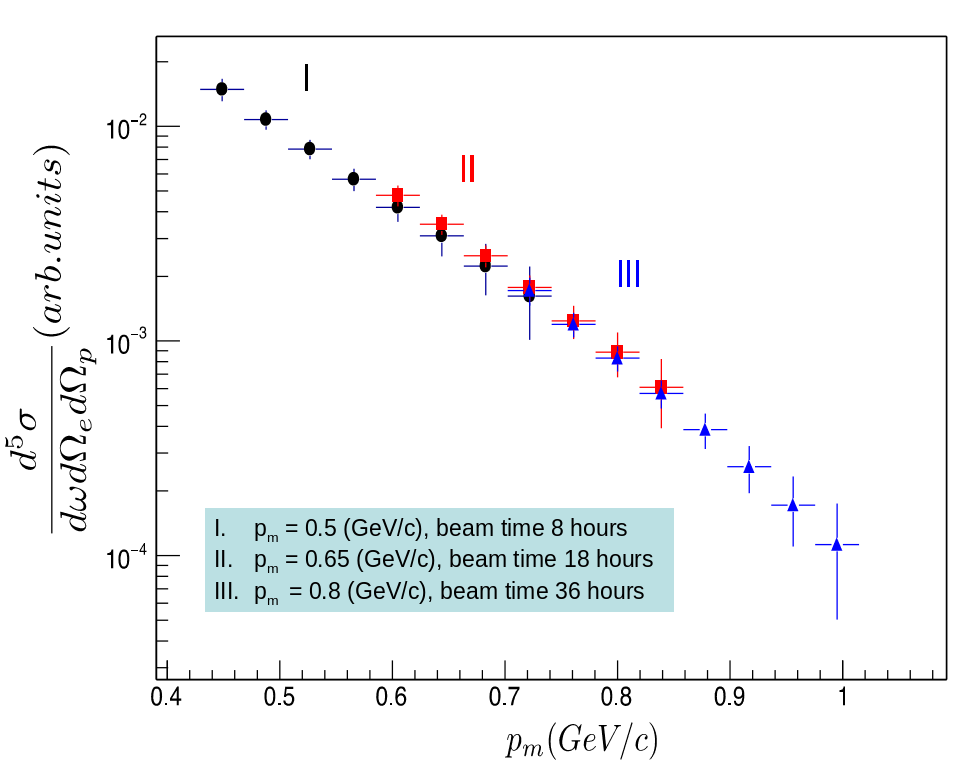
\includegraphics[width=3.2in, height=2.6in]{Exptd_Results.png}
  \caption{Expected D(e,e'p)n differential cross section as a function of missing neutron momenta for beam 
  energy/current of 10.6 GeV/c and 70 $\mu$A for E12-10-003.\cite{mark_pres}}
  \label{fig:Figure8}
\end{figure}
To satisfy the E12-10-003 kinematic requirements, the High Momentum Spectrometer (HMS) and Super HMS (SHMS) housed in Hall C will be set to
scattering angle and central momentum of $59.6^{\circ}\geq\theta_{p}\geq53.1^{\circ}$, $2.12\leq$ p$_{cent}\leq2.3$ GeV/c 
and $\theta_{e}=12.17^{\circ}$, p$_{cent}=$ 8.92 GeV/c, respectively. \\  
%Hall C is one of four
%experimental halls, each with its unique characteristics for performing a 
%variety of nuclear/particle physics experiments. Hall C in particular has
%two spectrometers, the High Momentum Spectrometer (HMS) and Super HMS (SHMS)
%(See Figure \ref{fig:Figure8}) 
% \begin{figure}[h]
%  \centering
% 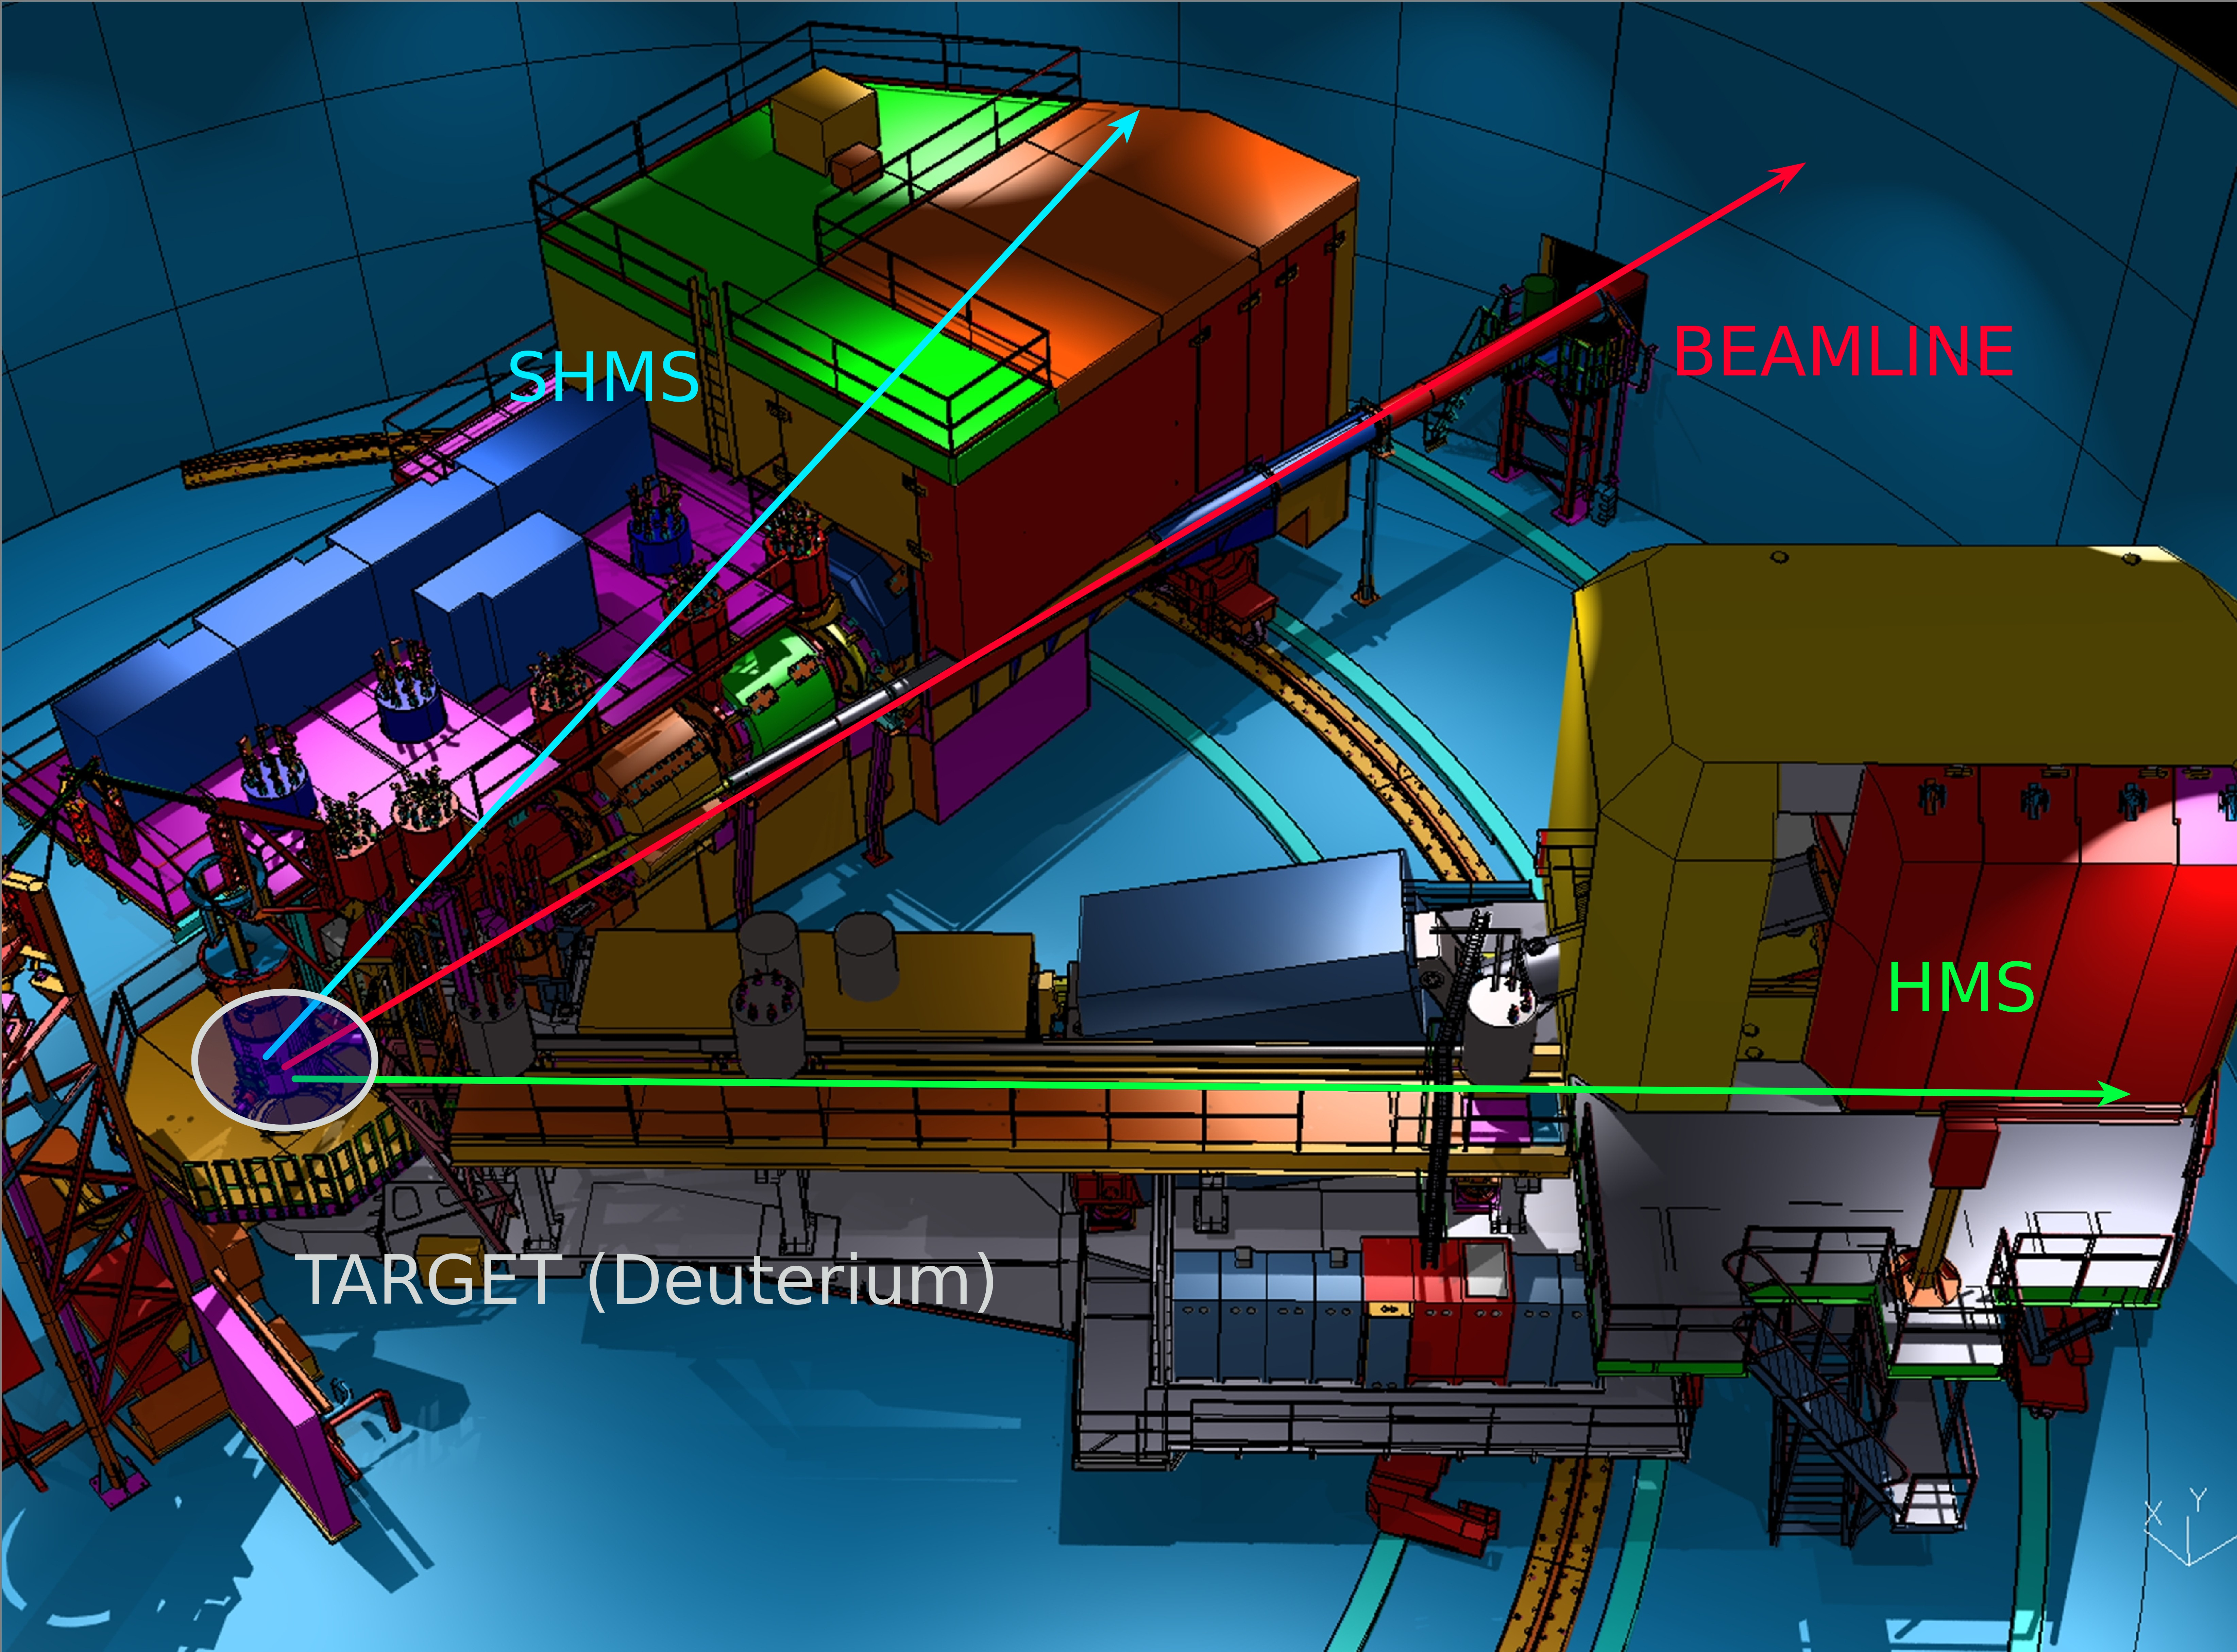
\includegraphics[width=2.7in, height=1.7in]{HMS_SHMS.jpg}
%  \caption{Artist view of HMS/SHMS at Hall C}
%  \label{fig:Figure8}
%\end{figure}
%Each spectrometer is composed by four magnets followed by a series of particle
%detectors serving their unique purpose. The magnets serve to steer the stream
%of particles produced following the interaction of the electron beam with the
%target. The detectors then gather information about the particles, such as 
%position, energy and time. This information is then analyzed through software
%in order to extract experimental observables (e.g. cross sections) that reveal
%the underlying physics processes of interest. \\
\indent Each spectrometer is comprised of a series of magnets followed by the detector stack (See Figure \ref{fig:Figure9}). The magnets
are set for a point-to-point tune and transport (focus) the scattered particles
to the detectors. The detectors are then read out by Analog- and Time- to Digital Convertors (ADC/TDC)(See p.281 of \cite{Leo}). 
\begin{figure}[h]
  \centering
  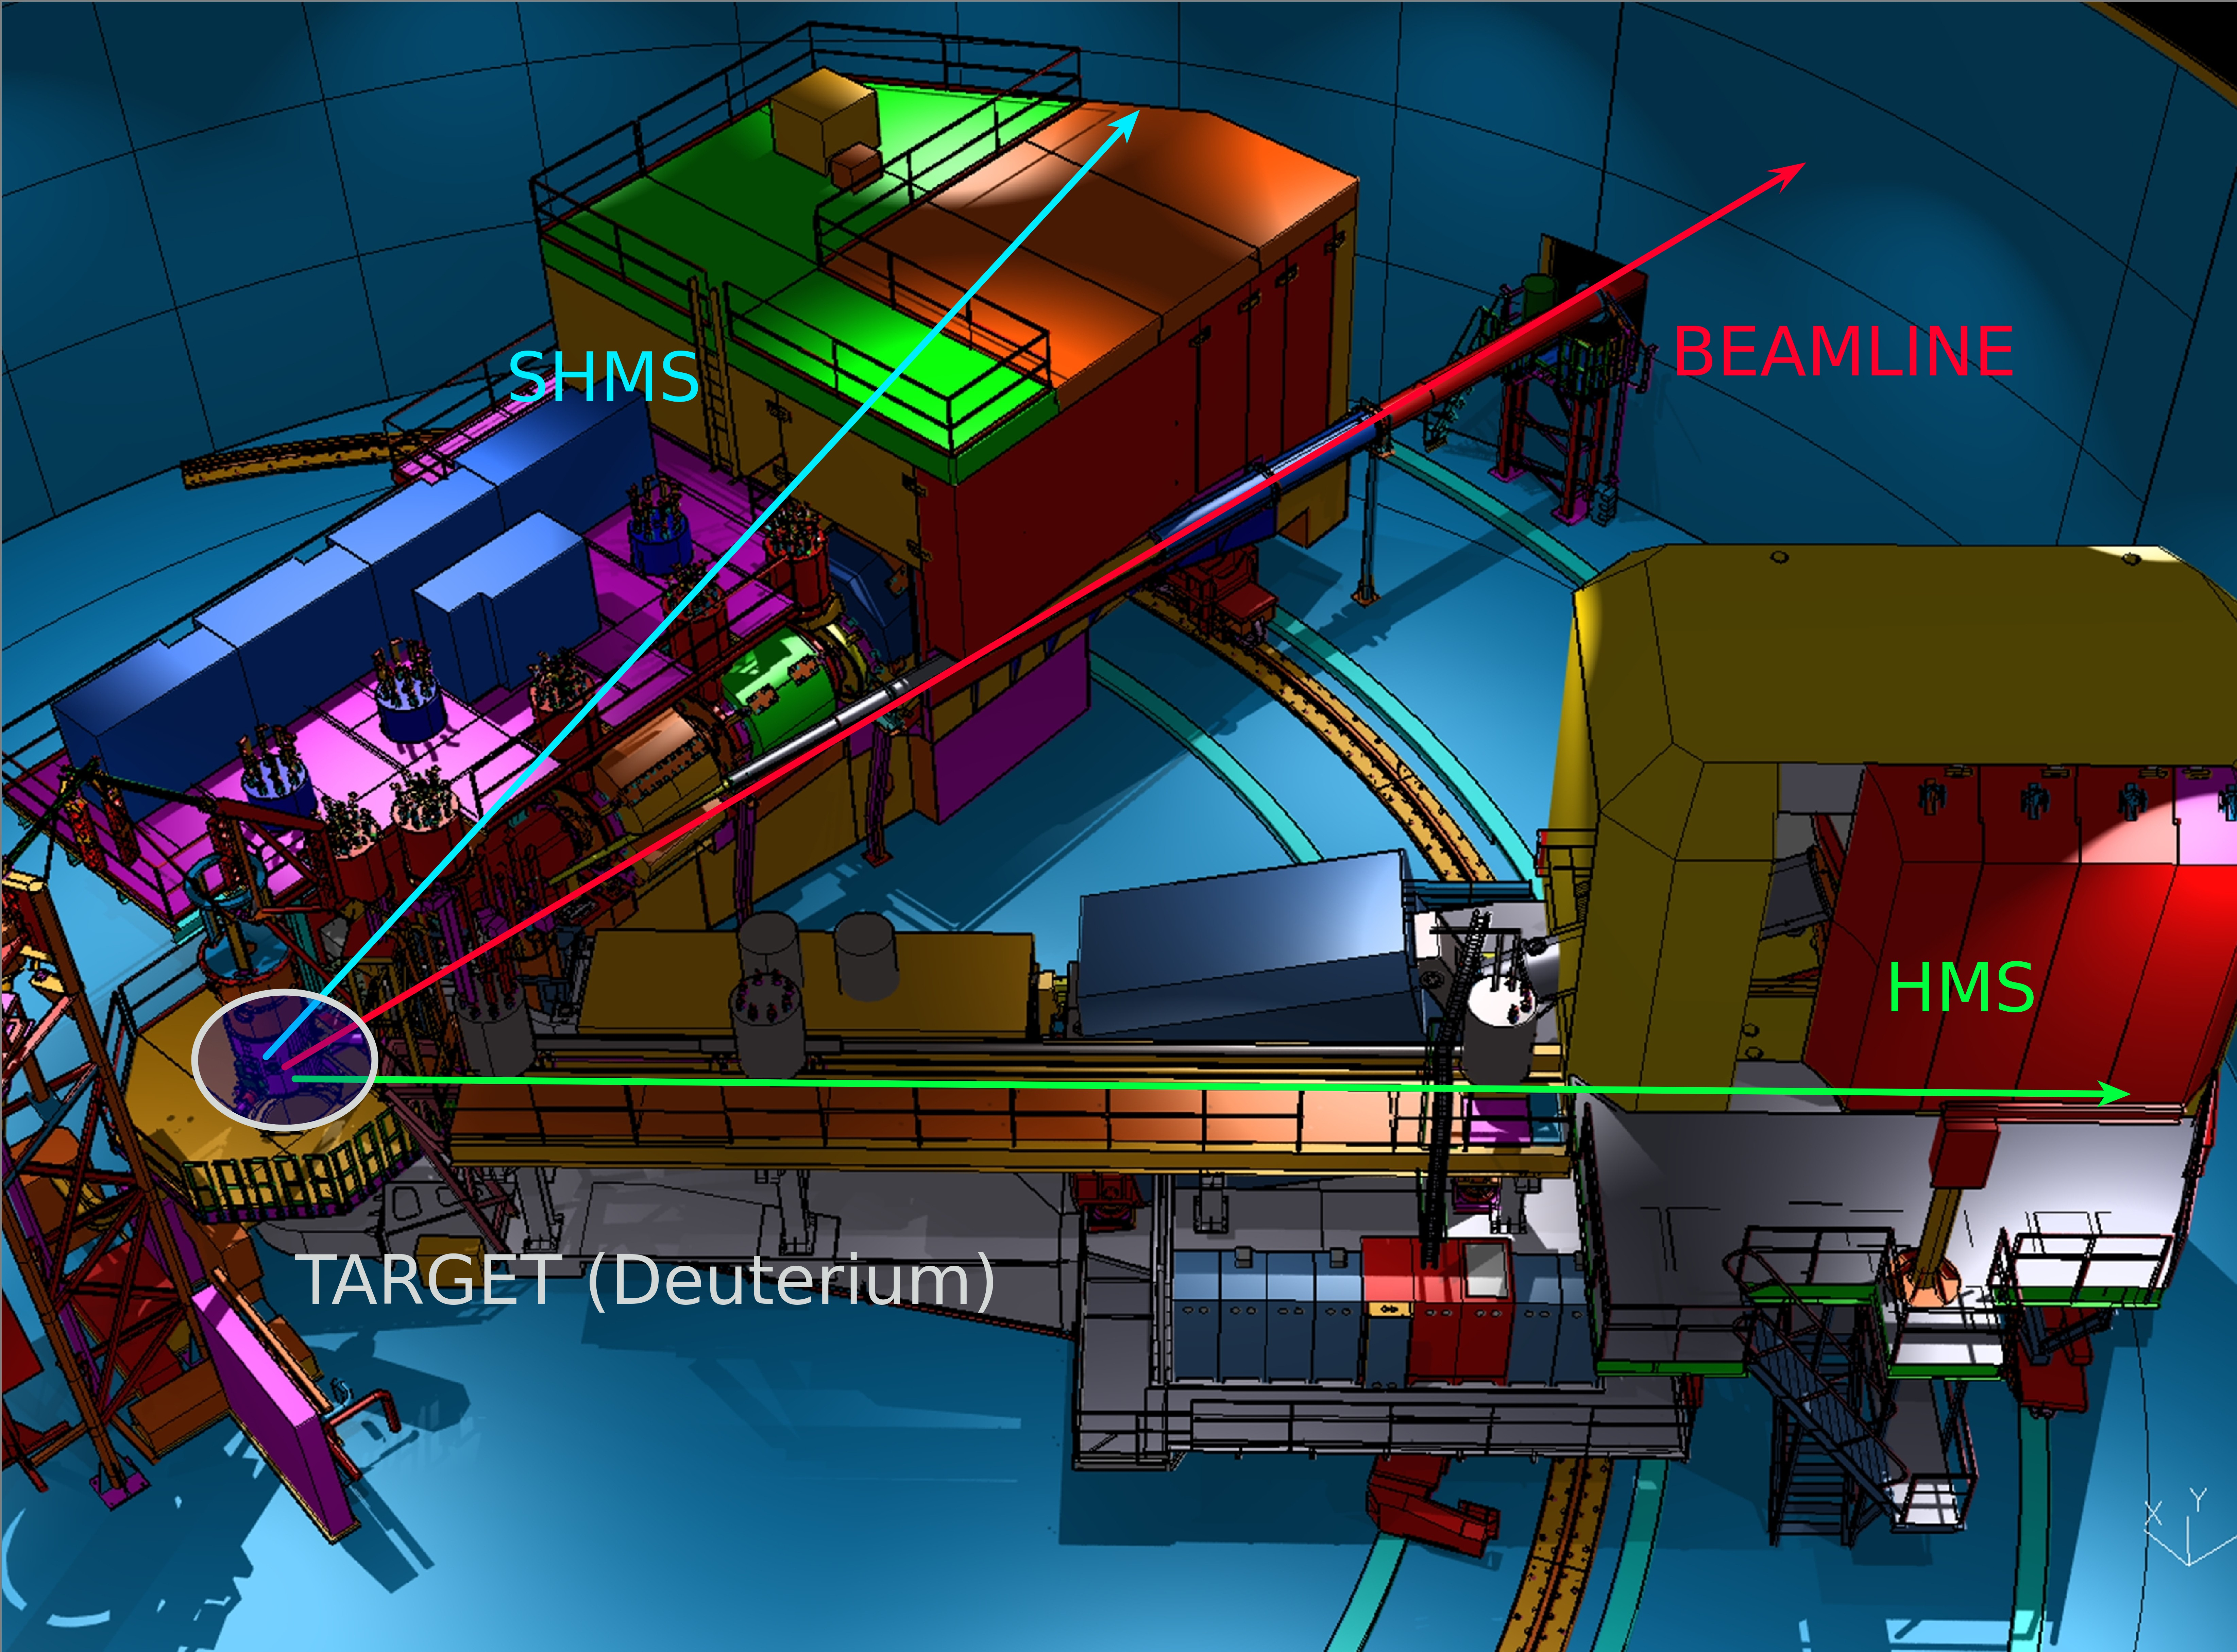
\includegraphics[width=3.0in, height=2.4in]{HMS_SHMS.jpg}
  \caption{Artist view of Hall C HMS/SHMS}
  \label{fig:Figure9}
\end{figure}
To extract meaningful information from the underlying physics, 
magnets and detectors (Hodoscopes, Wire Chambers, \v{C}erenkovs and Calorimeters) must be properly calibrated. \\ 
\indent The magnetic optics calibration main objective is to determine the transport matrix elements relating the
particle coordinates measured in the focal plane to those in the reaction vertex in the target. 
Knowledge of the matrix elements will provide a one-to-one mapping of measured particle tracks
to specific target location where the particle originated. \\
\indent Calibration of every detector element in the stack involves the translation of ADC/TDC hits
to equivalent energies  and times which are used to extract meaningful physics quantities.
Hodoscopes measure particle Time-of-Flight (TOF) from TDC values. These values must be corrected by
accounting for photon propagation time through the scintillator as well as pulse height, given that signals travelling
through a medium are attenuated.\\
\indent Drift Chambers measure particle position and must be calibrated to measure drift distance (distance between grounded sense wires and particle track).
Drift distances are determined from raw TDC hits registered by the sense wires and Hodoscope timing
information. \\ 
\indent Gas \v{C}erenkovs are used to discriminate particles based on threshold energies required to emit \v{C}erenkov radiation in the 
gas. The calibration of such detectors will involve isolating single photoelectron peaks in the ADC spectrum for each phototube.\\  
\indent Calorimeters measure energy deposition of particles and are able to discriminate between particles based on the
amount of energy deposited. To accurately measure energy deposited from raw ADC hits requires that the light attenuated
inside individual calorimeter lead blocks be accounted for. \\
\indent In addition to optics and detector calibrations, Beam Current Monitoring (BCM) and Target Boiling studies must be taken into consideration.
In E12-10-003, since a 15-cm long liquid deuterium target (T$_{\text{freezing}}$ = 18.7 K, T$_{\text{boiling}}$ = 25.3 K) needs to be cooled to 22 K, the power delivered by the beam can cause local
density fluctuations (local boiling) within the target, and so one needs to study the density fluctuations as a function of beam current in
order to correct for target boiling effects \cite{ibrahim}.\\   
\indent I am currently working on setting up a primary trigger in HMS/SHMS by
requiring 3/4 hodoscope planes in each spectrometer to fire (detect a hit) to consider the signal as 
a true event. The trigger then informs other detectors that the detected
signal is indeed a true event coming from the target. Once a primary trigger is set in
each spectrometer, a coincidence trigger (See p.287 of \cite{Leo}) needs 
to be set up between the HMS/SHMS in order to determine whether the detected particles originated
from the same interaction in the target. Depending on the nature of the experiment, additional triggers
may also be incorporated. \\
\indent I have also recently finished restoring one of the HMS Drift Chambers whose
exposure to radiation over a period of 25 years of use resulted in the
deterioration of 97 sense wires. All the broken sense wires
have been recently re-strung and tested. The chamber has been re-installed
in the HMS detector stack and we are currently taking a cosmic run to
monitor the detector response and diagnose any problems that may arise.

\newpage
\onecolumn
\bibliography{proposal}
\bibliographystyle{acm}


\end{document}
